To implement LessPM, we approached the development from a type-safety
environment.

\subsubsection{Server}
We chose Rust as the programming language for our backend, which provided
significant benefits regarding the software development environment.

Rust's emphasis on safety and performance allowed us to create a highly
secure and efficient environment for LessPM without the risks typically
associated with memory-related vulnerabilities~\cite{rivera2019preserving}.
The built-in memory management and focus on concurrency ensures that LessPM
ran smoothly, which is crucial~\cite{fischer1985impossibility} when
dealing with sensitive user data.

Additionally, Rust's surrounding ecosystem is at rapid
growth~\cite{librs-stats}, containing a vast library of high-quality
crates\footnote{
  \texttt{Crate} is the Rust-specific name for a package or library.
}, which enables expeditious development and easy integration of various
functionality.
Utilizing Rust's distinctive features, LessPM achieves enhanced security and
reliability in the context of user authentication~\cite{rivera2019preserving},
showcasing the benefits of utilizing a modern programming language.

LessPM ran an instance of an HTTPS server, serving as a wrapper for the
sensitive data.\footnote{
  We took advantage of the Authorization header during development, as specified
  in RFC 7519.
  However, the framework we used for the server required us to expose the usage
  of \texttt{Authorization header} to access it in the client.
  See Section~\ref{subsec:security-analysis} for further explanation.
}
The Chromium developers mandate the constraint of a secure connection to
guarantee that the pertinent Application Programming Interface (API) is invoked
exclusively within a secure context~\cite{webdev2021credential}.
During development, we established a secure connection by using a self-signed
certificate for the \texttt{``localhost''} domain.

As a deliberate decision, we opted for MongoDB due to its NoSQL architecture,
which facilitated the storage of Object-like structures~\cite{mongodb2021nosql}
including passwords, user accounts, and other related data that LessPM stores.

\subsubsection{Client}
An essential part of the implementation was to create a viable client that could
function as a visual entry point to LessPM and proof-of-concept.
For the simplicity of the project, we chose React as a framework.
React is a JavaScript library for building user interfaces, offering an
efficient and flexible approach to web development.
The design of LessPM was influenced by the principles of
least-knowledge~\cite{lieberherr1990assuring}, which underlined by the decision
to ensure that the LessPM client only retained necessary information to function
properly, containing no knowledge of LessPM's server nor its implementation.

We took advantage of React's ability to construct a single-page application with
no routing capabilities, avoiding the possibility of a malefactor utilizing URL
tampering or manipulation\footnote{
  Malefactors can perform URL Manipulation, which involves modifying a URL to
  request resources that would otherwise be inaccessible to a user.
} to attempt privilege escalation or accessing restricted data.

When initiating the project's development, we had a strong vision of creating
a client that could seamlessly integrate with Chromium-based browsers as
an extension.\footnote{
  In the client's project folder are traces of a manifest.json file and build
  scripts to have the client run in an extension.
}
However, we quickly discovered that the Rust cargo used to perform WebAuthn
requests did not implement this functionality.
We reported this issue
\href{https://github.com/kanidm/webauthn-rs/issues/288}{upstream to the authors}
of the cargo, and we will continue to work with the authors to ensure a proper
implementation of this functionality in the future.

LessPM's client maintains authentication and authorization through an
encrypted JSON Web Token (JWT, RFC7519), inspired by JSON Web
Encryption (JWE, RFC7516), passed back and forth between the server and client.


\subsection{Authentication \& Authorization}\label{subsec:auth-and-auth}
A system that maintains authentication and authorization through a stateless
protocol such as HTTPS, requires some information to authorize a
client between requested resources.
LessPM took advantage of JWTs and an inspired variation of JWEs for this
purpose.
Although JWTs are not inherently encrypted~\cite{RFC7519}, combined with JWE,
they serve as an essential backbone for secure data transfer in LessPM\@.

\subsubsection{JSON Web Tokens}
JWT is a compact, URL-safe string intended to transfer data between two
entities, often represented as a Base64 encoding.
They are often used as part of authentication and authorization scheme within
a web service, application, or API, and LessPM does this as well.
The data in the string is delivered as a payload and is referred to as a
\texttt{claim}~\cite{RFC7519}.

The JWT typically consist of three parts: header, payload, and signature.
The header and payload are serialized into JavaScript Object Notation (JSON)
and then encoded using Base64 to ensure a URL-safe format.
This permits larger bits of data to be sent in a compressed, safe\footnote{
  Safe in this context should not be interchanged with secure.
  We reference safe as a way to transfer the data over the selected protocol,
  in LessPM's case this HTTPS.
} format.

JWTs are widely used for scenarios such as single sign-on (SSO), user
authentication, and securing API endpoints by providing an efficient and
stateless mechanism for transmitting information about the user's identity
and permissions~\cite{karande2018securingnode}.
According to~\cite{RFC7519}, these should be attached to the
\texttt{Authorization} part of the HTTPS header, along with a hardcoded
\texttt{Bearer} part preceding the token, as the value of the header.

In LessPM, the JWT claim contained data we could use to validate and
authenticate a user between stateless HTTPS requests.
LessPM utilizes two functionalities of JWTs to ensure the validity of the
Base64-encoded token.

First, all tokens passed back and forth between the LessPM server and client
receives an expiry time.
We enforce this technique to ensure and maintain the security of accessed
resources, requiring a user to reauthenticate when the expiry timestamp is
passed.

Second, The tokens used in LessPM are cryptographically signed with RSA
Signature Scheme with Appendix - Probabilistic Signature Scheme (RSASSA-PSS)
using Secure Hashing Algorithms with 512-bit size (SHA-512), and is derived
from the Rivest-Shamir-Adleman (RSA) encryption.
The encryption is performed with a key-pair stored on LessPM's server to
mitigate the risk of token forgery and so LessPM can maintain the validity and
authenticity of the tokens created.
This prevents unknown authorities from constructing or hijacking tokens
belonging to LessPM\@.\footnote{
  Hijacking a token could happen by a man-in-the-middle attack.
  This is done by a third-party individual listening and intercepting traffic
  in order to either read data or input their own in a client's request.
  This would allow an attacker to gain access to privileged information.
}
Other signature algorithms that can be used include Hash-Based Message
Authentication (HMAC), Elliptic-Curve Digital Signature Algorithm (ECDSA), or
a plaintext secret stored on the server.
LessPM uses RSASSA-PSS with SHA-512 due to the asymmetric operations the
algorithms perform on the encryption and decryption, whereas HMAC and ECDSA is
based on symmetric- and elliptic curve cryptography.

\subsubsection{JSON Web Encryption}
By default, JWTs are not encrypted.
It is out of the question to unnecessarily expose any sensitive details about
LessPM's inner workings.
This lead to the decision of finding a way to encrypt the contents of the 
token before they are sent from LessPM's server.
Without the encryption, any malefactor could decode the Base64 encoding and
gain read access to the claim that LessPM uses to authorize and authenticate.

To perform this operation, LessPM seeks inspiration from JWEs and
RFC7516~\cite{rfc7516}.\footnote{
  To properly implement JWE, metadata should be encoded into the token, such as
  what algorithm performs the encryption~\cite{rfc7516}. For further
  explanation, see Section~\ref{sec:futurework}.
}

Before the RSASSA-PSS signed JWT is attached to the HTTPS header,
LessPM encrypted the Base64-encoded data using AES-256, before turning them into
a new Base64 encoded string.
Encrypting the token with AES-256 elevated the overall security of the
JWTs, making them more suitable for transferring sensitive data between the
intercommunicating entities in LessPM\@.

As a final step, the ciphertext created by AES-256 is again encoded into a
new Base64.
When LessPM again receives this claim, we used it to gather details about the
user who made the request and responded to the request accordingly.
An example of this encoding can be seen in
Appendix~\ref{subsec:base64-and-ciphertext}.

The process functions as follows in LessPM, and can also be seen in
Figure~\ref{fig:JWT-process}:
\begin{enumerate}
  \item The client completed an authentication request.
  \item A claim was constructed and created on the server.
  The claim could have been any data the server wished to use to authenticate
  the legitimacy of a future request.
  \item The claim was signed with the desired algorithm.
  This could also have been a secret, stored on the server.
  \item The claim is encoded into a Base64 string.
  \item The Base64 encoded string is passed to AES-256 encryption algorithm,
  creating a ciphertext.
  \item The cipertext is created into a new Base64-encoding, which is the
  final token.
  \item As part of the response to a request, the server appended the
  token.
  \item The client received the token and carried it upon the next performed
  request.
  \item When the server received the token again, it decodes the
  Base64-encoded ciphertext.
  \item The ciphertext is decrypted, decoded and reconstructed to a claim.
  \item The \texttt{exp} property of the JWT is validated and LessPM takes
  action accordingly.
\end{enumerate}

\begin{figure*}[htbp]
  \begin{center}

  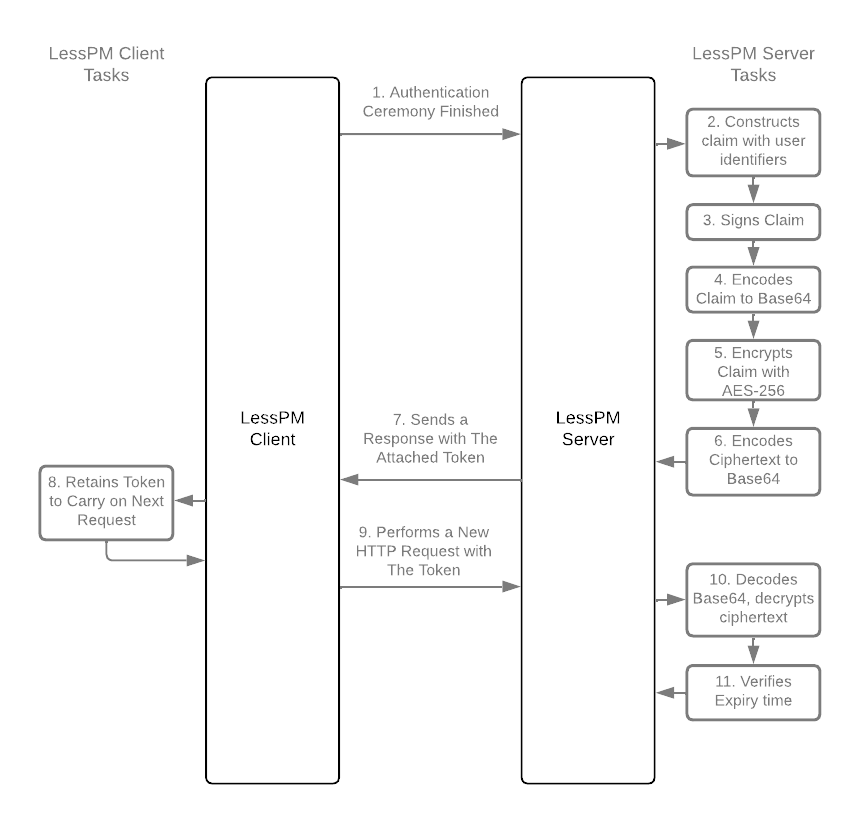
\includegraphics[scale=0.50]{images/JWT-JWE-process}
  \caption{The Process LessPM performs each time a token is initated.
  Starting with the finish of the Authentication Ceremony. The Y-axis depicts
  the time in which the actions are taken.}
  \label{fig:JWT-process}
  \end{center}
\end{figure*}

Further, the LessPM's server checked and verified the token before proceeding
with any requests made to it.
This information is updated and inspected between each
re-render~\cite{react-component} of LessPM's client.